\chapter{Background and Theory}

The achieved implementation consist of many different components including hardware (HW), advanced energy monitoring tools, Linux build systems and other software such as drivers. This section will elaborate on the specifics of the HW platform as well as the Linux build system and, the uClinux distribution and drivers necessary for controlling a Pong game with an external gamepad.

\section{EFM32GG}
The EFM32GG by Silicon Labs is a 32-bit MCU, and the best of its class in their range, based on its specifications \cite{SLABSMCUS}. It packs an ARM Cortex-M3 central processing unit (CPU), various peripherals, loads of general purpose IO (GPIO), 64–256 kB flash storage and 128 kB of RAM. One of the main advantages of using the EFM32GG, are the Energy Modes (EM) which are effective tools to control power consumption. \\

\section{DK3750}
The DK3750 development kit is a modular motherboard with detachable modules for a CPU board and different prototyping boards. The motherboard features buttons, LEDs, extra flash storage, extra RAM, an SD-card slot, Ethernet- and RS232-port, analog input and output jacks, a USB host connector, plenty of GPIO, and a 3.5" TFT-LCD display with a joystick.\cite{DK3750RM}

\section{Advanced Energy Monitoring}
Advanced Energy Monitoring (AEM) is a feature realized by the DK3750 board controller and the Silicon Labs software, Energy Profiler. It measures the MCU's current consumption in real-time. An option to show energy on the TFT-LCD display comes shipped with the kit. To enter this mode, just turn on the kit and push the appropriate button beneath the screen. 

\section{ARM Cortex-M3}
The ARM Cortex-M3 features a 3-stage pipeline-, Modified Harvard-, and RISC-processor architecture \cite{CORTEXM3RM}. A 3-stage pipeline is equivalent to the processor operating simultaneously on three instructions: One being fetched, another being decoded and the last being executed. Harvard architecture means having separate buses for instructions and data memory, enabling accesses to each space to happen concurrently. This greatly benefits performance. Reduced instruction set computing (RISC) architecture involves a process with a minimum number of instructions that can further make up other functions. \texttt{Load/store} are the only explicit instructions that references memory, all other instructions are handled inside internal registers. This, together with simple hardware (compared to CISC), is a core advantage of the RISC-architecture. When the three properties mentioned here are combined, they enable more work to be done in a single clock cycle, which further contribute to faster performance and a reduced demand for power. 

\section{Ptxdist Build System}

The Linux distribution is built with a build system called ptxdist. This system compiles and builds the kernel, the modules and other software programs. The results of the build is binary files that can be flashed to the development board. To use ptxdist it must be specified a configuration that defines the applications which are to be built for the HW platform. The setup is completed by specify a HW platform and the toolchain \cite{ptxsetup}. For more information on the workflow of ptxdist please refer to "Overview of ptxdist and build system - Lab Exercises in TDT4258 Energy Efficient Computer Systems" \cite{COMPENDIUM}.

\section{uCLinux}

uCLinux is a Linux distribution aimed specifically at small embedded computer systems. The kernel itself can use as little as 330K of flash, although this number usually exceeds a few megabytes when additional peripheral drivers are included . The distribution also needs a few megabytes of RAM to function properly. The EFM32GG is only equipped with 1MB of flash and 128kB of RAM, which is a little low to run uCLinux. However, the DK3750 has 16MB flash and 4MB of RAM connected to the EFM32GG through the external bus interface (EBI) \cite{DK3750RM}. By using this extra memory, the EFM32GG is able to run uCLinux with no problems.  

The main difference between a fully fledged Linux distribution and uCLinux is the lack of an memory managment unit (MMU). This makes the use of virtual memory (VM) impossible. When using VM, all of the processes run in the same virtual address space. This enables the possibility of using contiguous virtual memory, scattered physical pages and adding memory to an already running process.

With no VM, all memory allocated to a process must be contiguous. This might cause fragmentation problems, especially for configurations that spawns many processes dynamically. Luckily, embedded systems often tend to have static process, which mitigates the fragmentation problem of not having an MMU.   

\section{Framebuffer}

The LCD display on the DK3750 was used for this project. The LCD display has a resolution of 320x240 pixels, and a color depth of 16-bit. The display can either be driven by the on-board SSD2119 display controller, or by using direct drive mode from the EFM32GG. In both cases, data is sent as 16-bit RGB format. The data is organized as shown in Figure \ref{fig:display_format}. 

\begin{figure}[h]
\centering
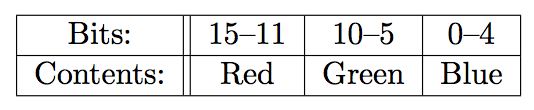
\includegraphics[width=0.6\textwidth]{images/display_format.png}
\caption{Organisation of each pixel in the framebuffer. \cite{COMPENDIUM}}
\label{fig:display_format}
\end{figure}

A pre-made Linux device driver was used to communicate with the display. The device driver utilizes a frame buffer, as depicted in Figure \ref{fig:framebuffer}. A simple API was implemented in ANSI C for this driver. The API features functions for drawing simple geometric shapes and text on the display.  

\begin{figure}[h]
\centering
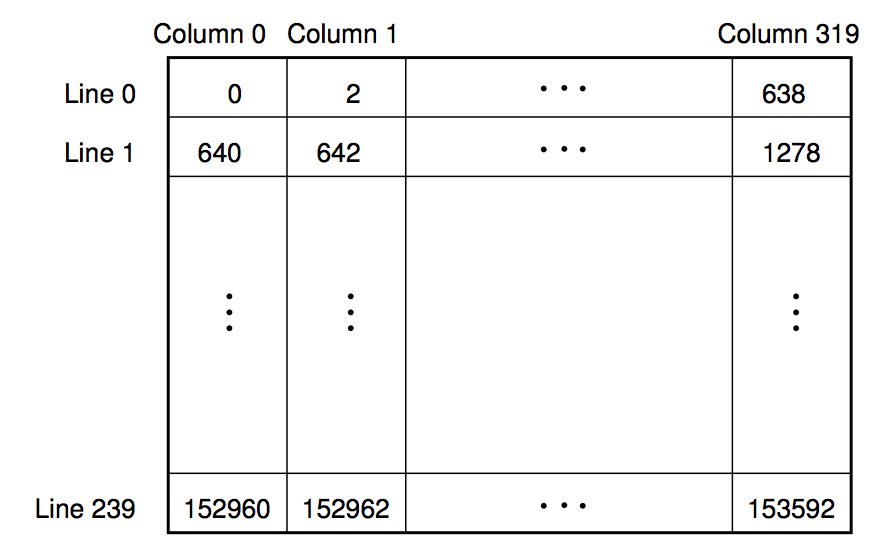
\includegraphics[width=0.6\textwidth]{images/framebuffer.png}
\caption{Organisation of ramebuffer. Each square corresponds to one pixel and the address of this pixel. \cite{COMPENDIUM}}
\label{fig:framebuffer}
\end{figure}


%Loadable kernel module
%Interface between kernel and module
%Ptxdist

\section{Device Drivers}

This section is an introduction to the fundamentals of a device driver, especially Linux device drivers, and how a char device driver is implemented in a Linux environment. It will also elaborate on how interrupts can asynchronously notify processes through a device driver.

\subsection{What is a Device Driver?}

A device driver \cite{devicedriver} is a software program which delivers an interface between operating systems (OS) and HW devices connected to it. This is convenient when programs run by the OS should access the HW and don't have to bother with complex HW functions and memory allocation. From the OS's point of view there should be a ``black box'' between its interface and the HW.

\subsection{Linux Device Drivers}

In the Linux environment device drivers are implemented as modules which is a piece of code added to the kernel at runtime \cite{module}. This module defines the driver methods, registers the driver, allocates an appropriate memory region for the device and handles the HW functions \cite{ch3}. Driver methods are the functions available for the invoker of the driver. When registering a driver, different entries for the driver are made in the file system, and especially the driver could be made available in User Space in the \emph{/dev} directory.

Different device drivers are often put in three classes \cite{classes}: \emph{Char device, Block device and Network interface}. This report will focus on the Char device as this was implemented in the final solution. 

\subsection{Char Device Drivers}

%A Char device is a device that needs to be accessed in a byte stream oriented way \cite{classes}. 

The setup of a char device driver consists of a routine to be executed when loaded and unloaded from the kernel. This is achieved through an \emph{init} and \emph{exit} function \cite{initexit} inside the driver. The \emph{init} function includes most of the setup for communicating with the device and creating the device in the kernel file system. The \emph{exit} function ensures that the driver is completely removed from the kernel and all structures and memory regions are released. 

One of the most important structures inside the driver is the file operation structure \cite{fops}. This structure holds the methods of the driver such as \emph{open, close, release, write} and \emph{fasync}. The methods \emph{open, close, release} and \emph{write} handles the system calls \emph{open, close, read} and \emph{write}. This lets applications in user space access the driver through shell command as \emph{echo} or \emph{cat}, in example. The \emph{fasync} \cite{fasync} method enables asynchronous notification between the driver and the invoking process. 

Since the creation of the device happens in the \emph{init} function there are a few necessary steps which must be included in this function. First the device is registered to the kernel and assigned a major number so that the driver can be identified to a device \cite{major}. Calling the function \texttt{alloc\_chrdev\_region} \cite{region} registers the device and dynamically allocates a major number for use through the creation of the device. In order to create the device a class structure has to be initialized with the function \texttt{class\_create} \cite{class}. Now the device can be created by calling \texttt{device\_create} \cite{devcreate} and passing a pointer from the class structure as an input parameter. The device is then initialized and added to the kernel with the \texttt{cdev\_init} \cite{cinit} and the \texttt{cdev\_add} \cite{cadd} functions. Now the device is created in the kernel file system and the driver instance is found in the \emph{/dev/} directory. Additional setup, such as requesting memory for the device, is also to be put in the \emph{init} function.

When the driver is unloaded from the kernel the call to the \emph{exit} function must ensure the release of all the resources setup for the device. The \emph{exit} function should therefor delete the device and the class structure with the functions \texttt{device\_destroy} \cite{devdestroy} and \texttt{class\_destroy} \cite{classdestroy}. Before unregistering the char device with function \texttt{unregister\_chrdev} \cite{unregister} the cdev structure is deleted with the function \texttt{cdev\_del} \cite{cdel}.

For the driver to support interrupts through asynchronous notification an interrupt handling function and a function for the method \emph{fasync} is needed. All the necessary memory allocation and setup of interrupts are done in the \emph{init} function, but the signaling procedure are put in the interrupt handler. A call to the function \texttt{kill\_fasync} \cite{fasync} will signal the interested process of the occurrence of the interrupt. The \texttt{fasync\_helper} \cite{fasync} function is put in the \emph{fasync} method to register interested processes for asynchronous notification. To invoke this method the user space program must implement the code:

\begin{lstlisting}
    int oflags;
    descr = open("/dev/some-driver", O_RDONLY);
    signal(SIGIO, &interrupt_handler);
    fcntl(descr, F_SETOWN, getpid());
    oflags = fcntl(descr, F_GETFL);
    fcntl(descr, F_SETFL, oflags | FASYNC);
\end{lstlisting}

It is possible to copy memory of the device to user space by calling the function \texttt{copy\_to\_user} \cite{cpyusr}. This is often called when the \emph{read} method is called. 

%A Char device driver often implements functions for the four system calls \emph{open, close, read and write} which are used for communicating with the device. The driver also functions as a link between Kernel Space and User Space. The driver must implement a way to grant the request of Kernel Space data if it is intended by the driver to provide this for the User programs. 

%\subsection{Advanced Char Device Drivers}

%More advanced drivers provides more functionality as interrupt handling and asynchronous notification of other processes \cite{ch3}. 

\section{Pong}

Pong is a two-dimensional, table-tennis inspired arcade game, initially developed by Allan Alcorn, and released by Atari in 1972. It was a huge commercial success, and is considered to have had a great contribution towards the rise of the video game industry. 

The game 